%____________________________________________________________________________||
\section{Event selection and categorisation for signal and control regions}
\label{sec:selection}

This section first outlines the set of ``pre-selection'' requirements
that are common to all signal and control regions, before defining the
selection criteria that are specific to each region.

%%____________________________________________________________________________||
\subsection{Pre-selection}
\label{sec:preSelection}

\subsubsection{MET filters}

A number of beam- and detector-related effects can induce significant
\met. Examples include beam halo, reconstruction failures, spurious
detector noise, or event misreconstruction due to detector
inefficiencies. These events, with large, non-physical values of \met,
are rejected with high efficiency by applying a range of dedicated
vetoes. All ``MET filters'' recommended by the JetMET POG and SUSY PAG
are applied by default in this analysis and listed in Table~\ref{tab:pre-selections}.

\subsubsection{Jet requirements}

Jets considered in the analysis are required to satisfy $\PT>40\gev$
and $|\eta|<2.4$. Events containing jets in the forward region that
satisfy the requirements $\PT>40\gev$ and $|\eta|>2.4$ are rejected (regardless of the identification requirement) 
in order to control background contributions from SM processes, without
introducing a significant reduction in signal acceptance. The selected jets 
are used in the calculation of all jet-based
event-level variables, such as \HT, \mht, and \alphat.

The lead jet is required to satisfy $\PT > 100\gev$. 
This helps to ensure high trigger efficiencies,
but also helps to improve the S/B for a wide
range of models with respect to SM processes, such as V + jets
production. Events are then classified based on the
second leading jet. In the case that a second leading jet satisfies $\PT > 100\gev$ 
events are assigned to a ``symmetric'' \njet category. If the second
jet satisfies $40 < \PT < 100\gev$ events are assigned to an
``asymmetric'' \njet category. Finally, if there is no other jet 
with $\PT>40\gev$, events are assigned to the ``mono-jet''
category. This categorisation is heavily utilised throughout all the document. \\
The asymmetric and mono-jet categories have been added to
the analysis to help improve acceptance to a range of DM models and compressed
SUSY.

\subsubsection{Jet-based energy sums}

Events are required to have significant hadronic activity by requiring
$\scalht > 200\GeV$. Despite an increase in both multijet production
cross sections and pileup in Run~2, the lowest \HT threshold is
kept at the same value of the Run~1 analysis~\cite{Chatrchyan:2013lya}
in order to maintain acceptance to DM models or compressed
SUSY. 

An estimator of the missing transverse energy for each event, \ETmiss,
is determined from the vectorial sum of the jet transverse momenta,
known as \mht. Events are required to have appreciable missing
transverse energy by requiring $\mht>130\gev$. This requirement is
applied to events in the signal and control regions. The
\scalht-dependent \alphat thresholds, required to suppress multijet
events as outlined in Sec.~\ref{sec:had-signal}, provide an effective
threshold on \mht comparable to 130\GeV via the relationship in
Eq.~(\ref{eq:alphat3}). Hence, the extrapolation from control to
signal region in \mht is minimal. 

\subsubsection{The \mht/\met variable}

Finally, the value of \mht is compared to the missing transverse
energy variable, $\met$. Only events that satisfy
$R_{\mathrm{miss}}=\mht/\met < 1.25$ are considered in order to
protect against events containing multiple jets outside the
experimental acceptance that contribute significantly to \mht. In the
case of the control regions, in which well-reconstructed, isolated
muons and photons are selected, the $R_{\mathrm{miss}} < 1.25$
requirement is also applied. The \mht sum does not consider the
transverse momentum of the muons or photon. Hence their momenta are
also added to the \met such that the \mht and \met can be considered
on an equal footing.

The pre-selection requirements are summarised in Tab.~\ref{tab:pre-selections}

\begin{table}[h!]
  \topcaption{Summary of the pre-selection criteria.}
  \label{tab:pre-selections}
  \centering
  \footnotesize
  \begin{tabular}{ ll }
    \hline
    \hline
    Selection                     & Requirement                                                                          \\
    \hline
    ``MET filters''               & \parbox[t]{10cm}{Primary Vertex, CSC Beam Halo,
      HBHE Noise and Isolation, \\ ECAL Endcap SC Noise, ECAL TP, Bad
      Muon, Bad Charged Hadron}         \\
    Jet acceptance                & $\PT > 40\gev$, $|\eta| < 2.4$                                                         \\
    Lead jet acceptance           & $\PT > 100\gev$, $|\eta| < 2.4$                                     \\
    Forward jet veto              & $\PT > 40\gev$, $|\eta| > 2.4$                                     \\
    \HT requirement               & $\HT > 200\gev$                                                        \\
    \mht requirement              & $>130\gev$                                                     \\  
    \hline
    \hline
  \end{tabular}
\end{table}

\subsection{The hadronic signal region}
\label{sec:had-signal}

\subsubsection{Lepton, photons and SIT vetoes}
\label{sec:vetoes}
Using the identification criteria described in Sec.~\ref{sec:objects}, 
the following objects are vetoed when selecting events for the hadronic signal region:
\begin{itemize}
\item muons with $\pt>10\,\mathrm{GeV}$ and $|\eta|<2.5$;
\item electrons with $\pt>10\,\mathrm{GeV}$ and $|\eta|<2.5$;
\item single isolated tracks with $\pt>10\,\mathrm{GeV}$ and $|\eta|<2.5$;
\item photons with $\pt>25\,\mathrm{GeV}$ and $|\eta|<2.5$;
\end{itemize}


\subsubsection{\alphat requirements}
\label{sec:HT-AT-selection}

After the pre-selection criteria and the vetoes are applied, 
the multijet background is still several orders
of magnitude larger than the typical signal expected from SUSY.
Background events from multijet production populate the region
$\alphat \lesssim 0.5$ and therefore can be rejected with very high
efficiency by requiring an appropriate cut on \alphat. \\
The cut on \alphat is chosen in order to ensure a trigger efficiency close to unity 
in all the bins. More details on the trigger strategy can be found in Sec.~\ref{sec:triggers}.\\
Table~\ref{tab:alphat-thresholds} summarises the 
\alphat thresholds for each \HT bin. 
The \alphat threshold is dependent only on \HT and not
on \njet nor \nb that are used to define the event categories. \\
No \alphat cut is applied in the monojet bins, as the variable is defined only for $\njet\geq2$. 

\begin{table}[h!]
  \caption{\alphat thresholds versus
    lower bound of \scalht bin. For all \HT bins satisfying $\HT >
    900\gev$, no \alphat cut is applied. No \alphat requirement is
    imposed in the monojet bins.}
  \label{tab:alphat-thresholds}
  \centering
  \footnotesize
  \begin{tabular}{ lccccccccc }
    \hline
    \hline
    \scalht            & 200       & 250       & 300       & 350       & 400       & 500       & 600 &  $>$900    \\
    \hline                                                                                     
    \alphat threshold  & 0.65      & 0.60      & 0.55      & 0.53      & 0.52      & 0.52      & 0.52 & --    \\
    \hline
    \hline
  \end{tabular}
\end{table}


\subsubsection{\bdphi requirement} 
\label{sec:bdphi-selection}

Further, an additional powerful variable \bdphi is used to suppress
multijet contamination due to both instrumental effects and
semi-leptonic heavy-flavour decays with genuine \met in the final
state. The variable is determined as follows. The jet-based estimate
of the missing transverse energy, ${\mhtvec}$, is determined from all
jets ($\mathrm{j}_i \,\in\, [1,\njet], \mathrm{j}_i \ne \mathrm{j}_k$)
except for one of the reconstructed jets (the ``test'' jet
$\mathrm{j}_k$). The difference in the azimuthal angle between the
recomputed $\mhtvec$ and the ``test'' jet is then determined. This
process is repeated for each jet $\mathrm{j}_i$ in the event and the
minimum of all the azimuthal differences, \bdphi, is determined.:

\begin{equation}
  \bdphi = \min_{\,\forall\, \mathrm{j}_k\,\in\, [1,\njet]}
  \Delta\phi \Bigl( \ptvec^{\,\mathrm{j}_k}, \,
    -\hspace{-0.5em}\sum_{\substack{\mathrm{j}_i= 1 \\ \mathrm{j}_i \ne \mathrm{j}_k}}^{\njet}
    \ptvec^{\,\mathrm{j}_i} \Bigr).
  \label{eq:bdphi}
\end{equation}

For monojet events, the calculation is performed using all jets with
$\Pt > 25\gev$, with the variable identified as $\bdphilow$.

The ``test'' jet corresponding to \bdphi is 
identified as the jet that is most likely to have given rise to the
missing transverse energy in the event. Events with significant \mht
due to instrumental effects or heavy flavour decays populate the
region at $\bdphi$ and so candidate signal event are accepted
only if they satisfy $\bdphi > 0.5$. The use of the \bdphi and \alphat
variables provide an extremely powerful rejection factor against
contamination from multijet events and allow to maintain low jet \PT,
\HT, and \mht thresholds, which in turn maximises signal acceptance
for a large range of DM and SUSY models with final states
characterised by the presence of significant \met.

  
\subsubsection{Beam halo}
\label{beam-halo-selection}

The CSC beam halo filter has been found to be less efficient during the early
Run 2 data-taking period compared to the previous run.

Beam halo events manifest themselves as single energy deposits in the
calorimeters, which introduces large amounts of ``fake'' \met. This effect is
especially prominent in the signal region monojet category, particularly at
$\phi$ coordinates of 0 and $\pi$ because of the tendency of halo particles to
lie within the plane of the LHC ring. 

Such spurious events are suppressed by requiring at least 10\% of the leading
jet's energy to originate from charged hadrons, $CHF>0.1$. The effectiveness of this selection
is demonstrated in Fig.~\ref{fig:leadJetCleaning}.

There is no need for this selection in the control regions, 
as the requirement of well identified physics objects, like muons 
and photons naturally removes spurious events of this kind. 

This cut can be regarded as 
an additional tight jet ID requirement employed in the analysis, 
with efficiency close to one for real jets and thus not affecting the 
signal efficiency significantly. 


\begin{figure}[h!]
    \begin{center}
        {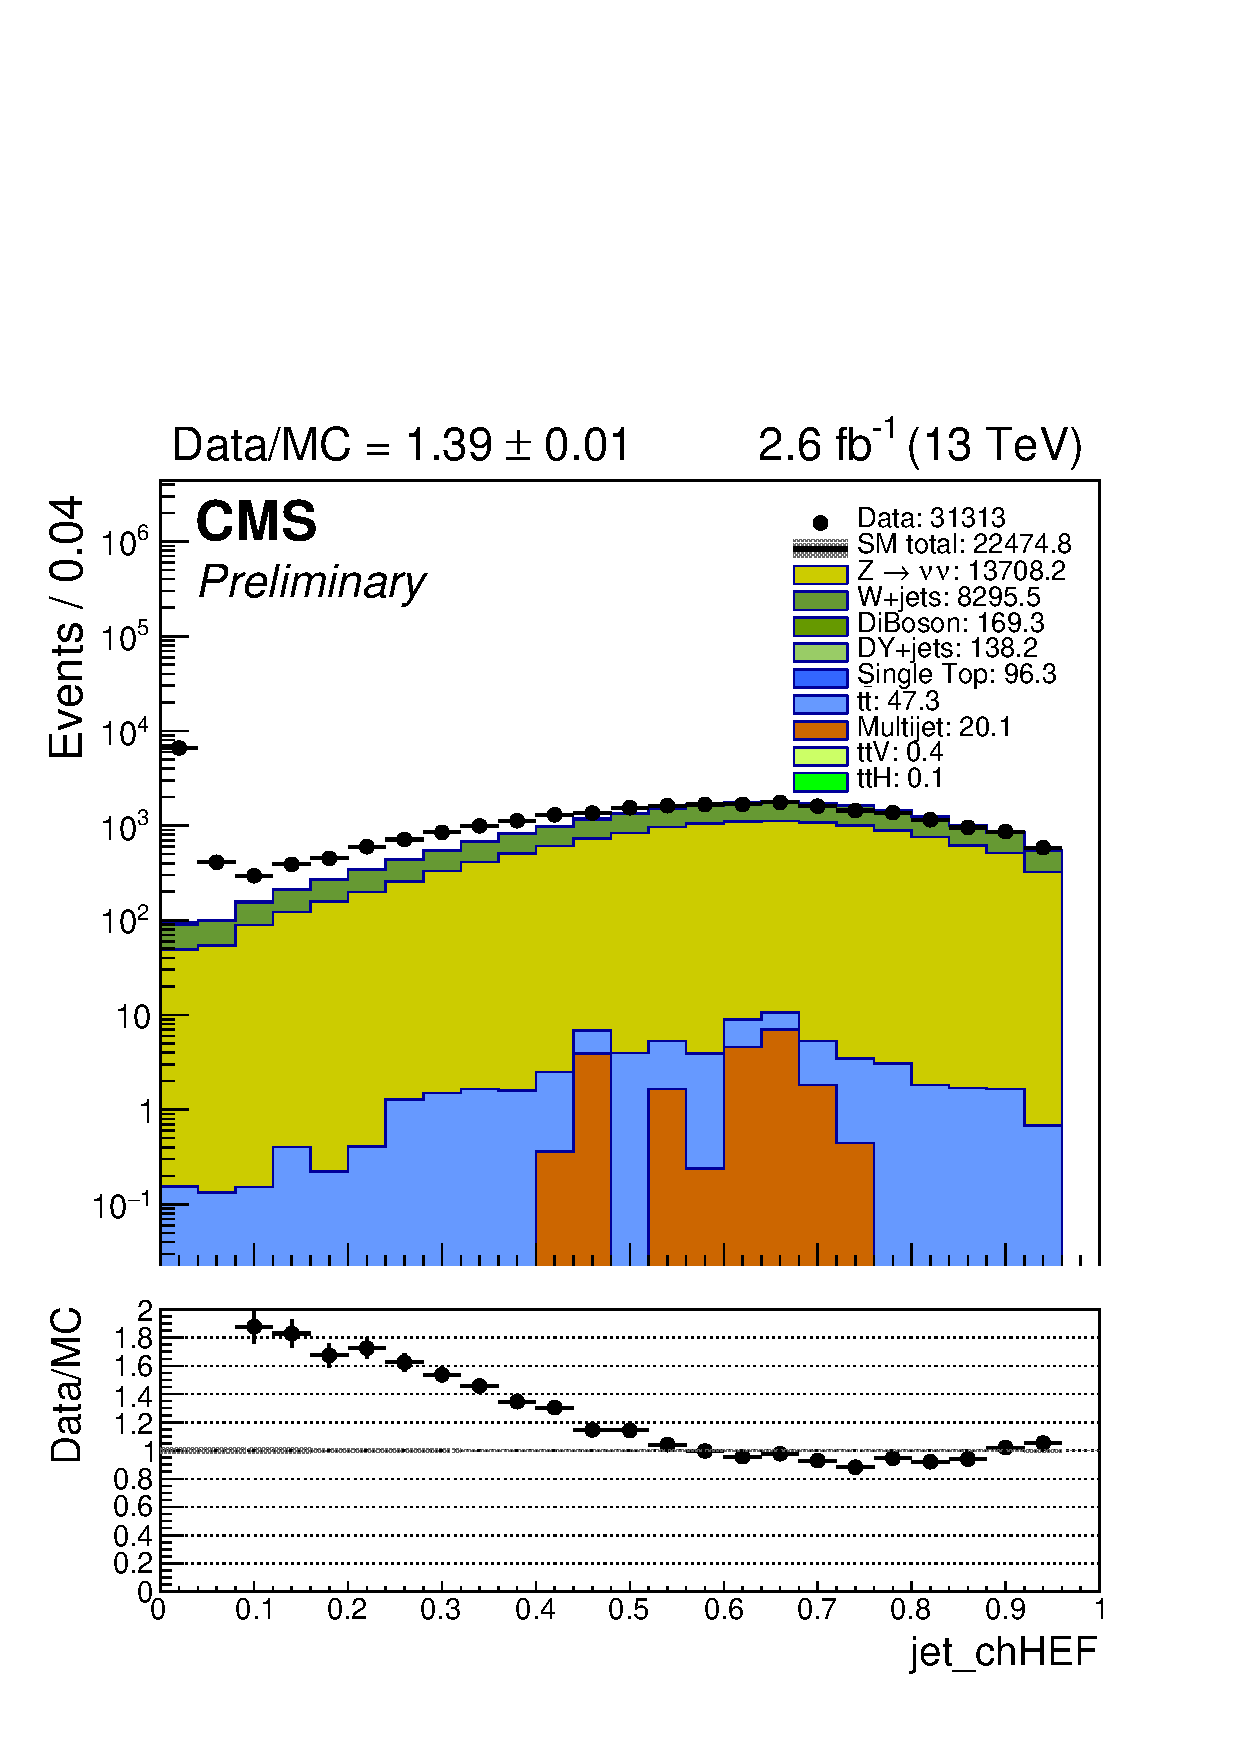
\includegraphics[width=0.32\textwidth]{figures/selection/jet_chHEF_mono_all_before.pdf}}
        {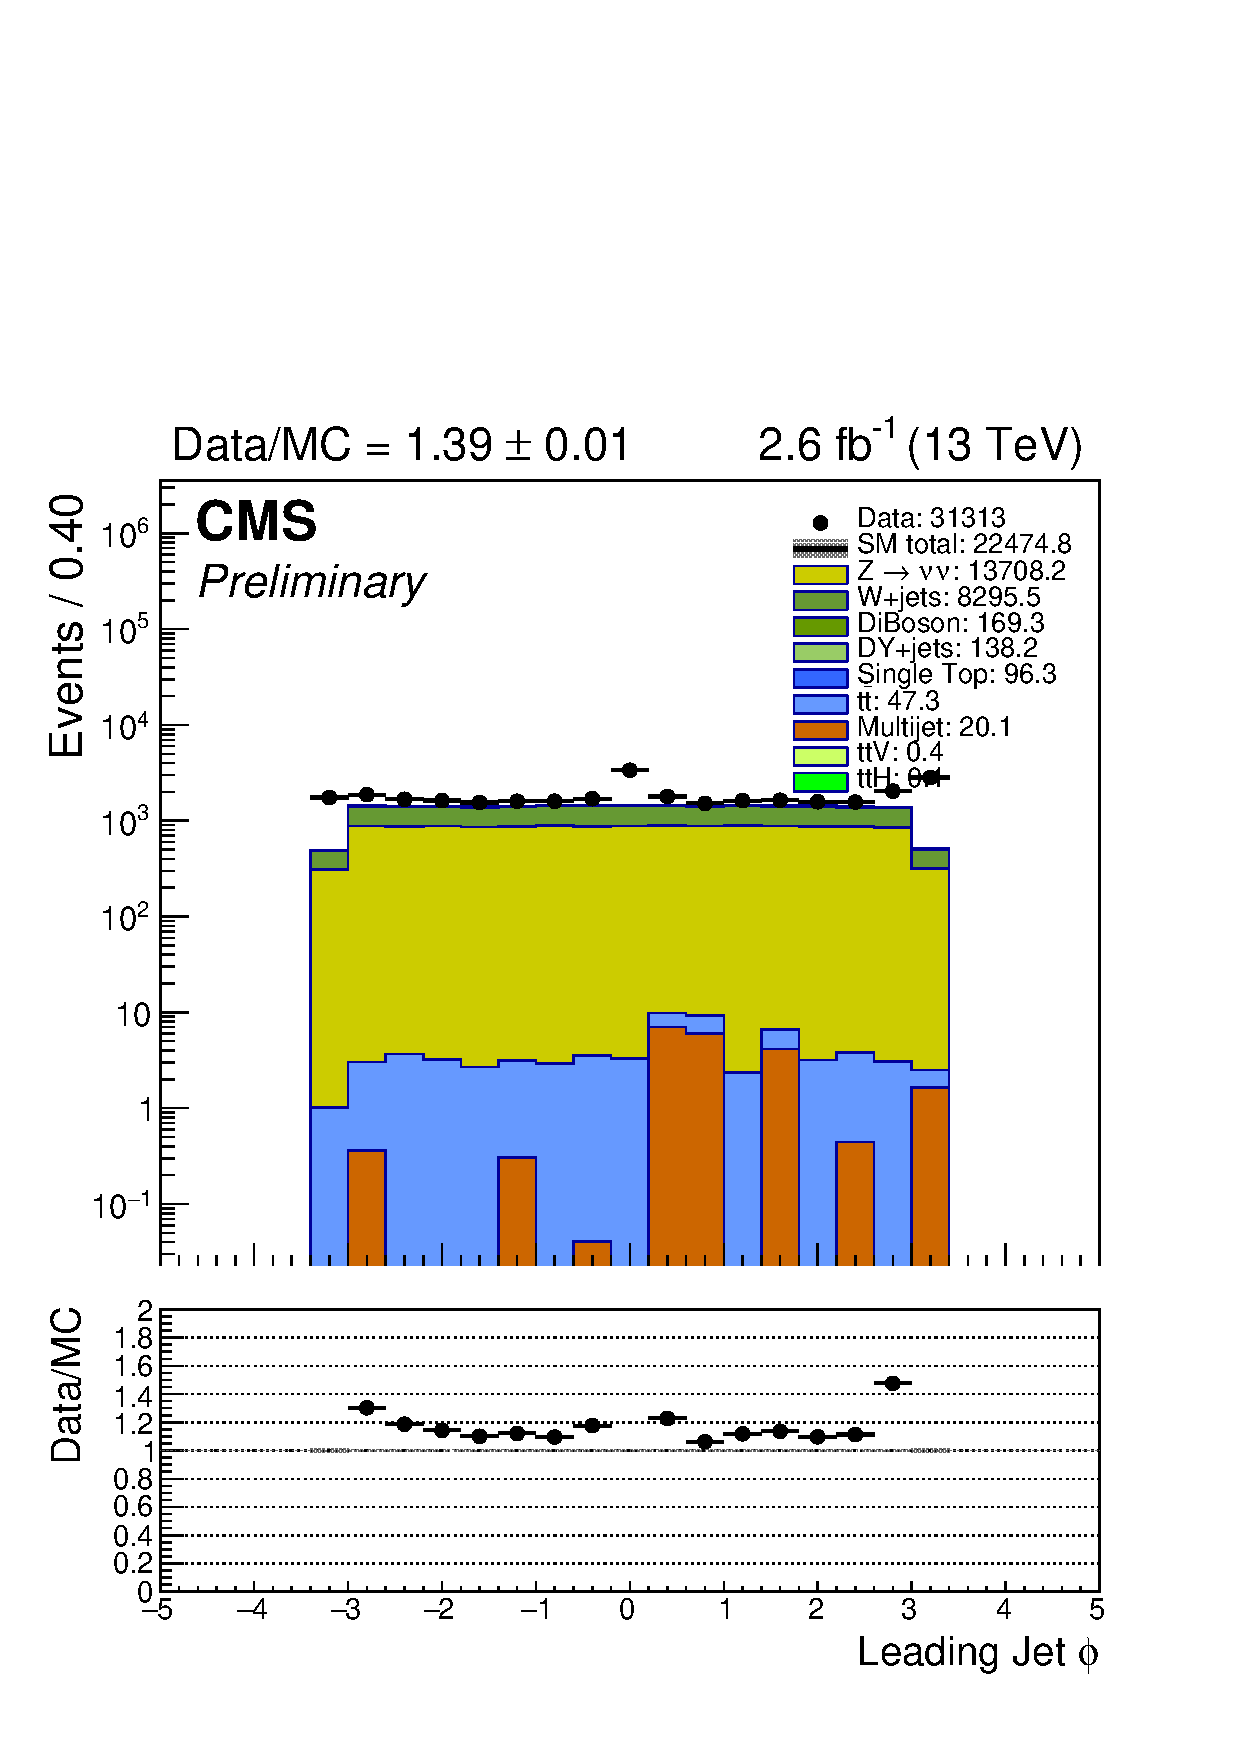
\includegraphics[width=0.32\textwidth]{figures/selection/jet_phi[0]_mono_all_before.pdf}}
        {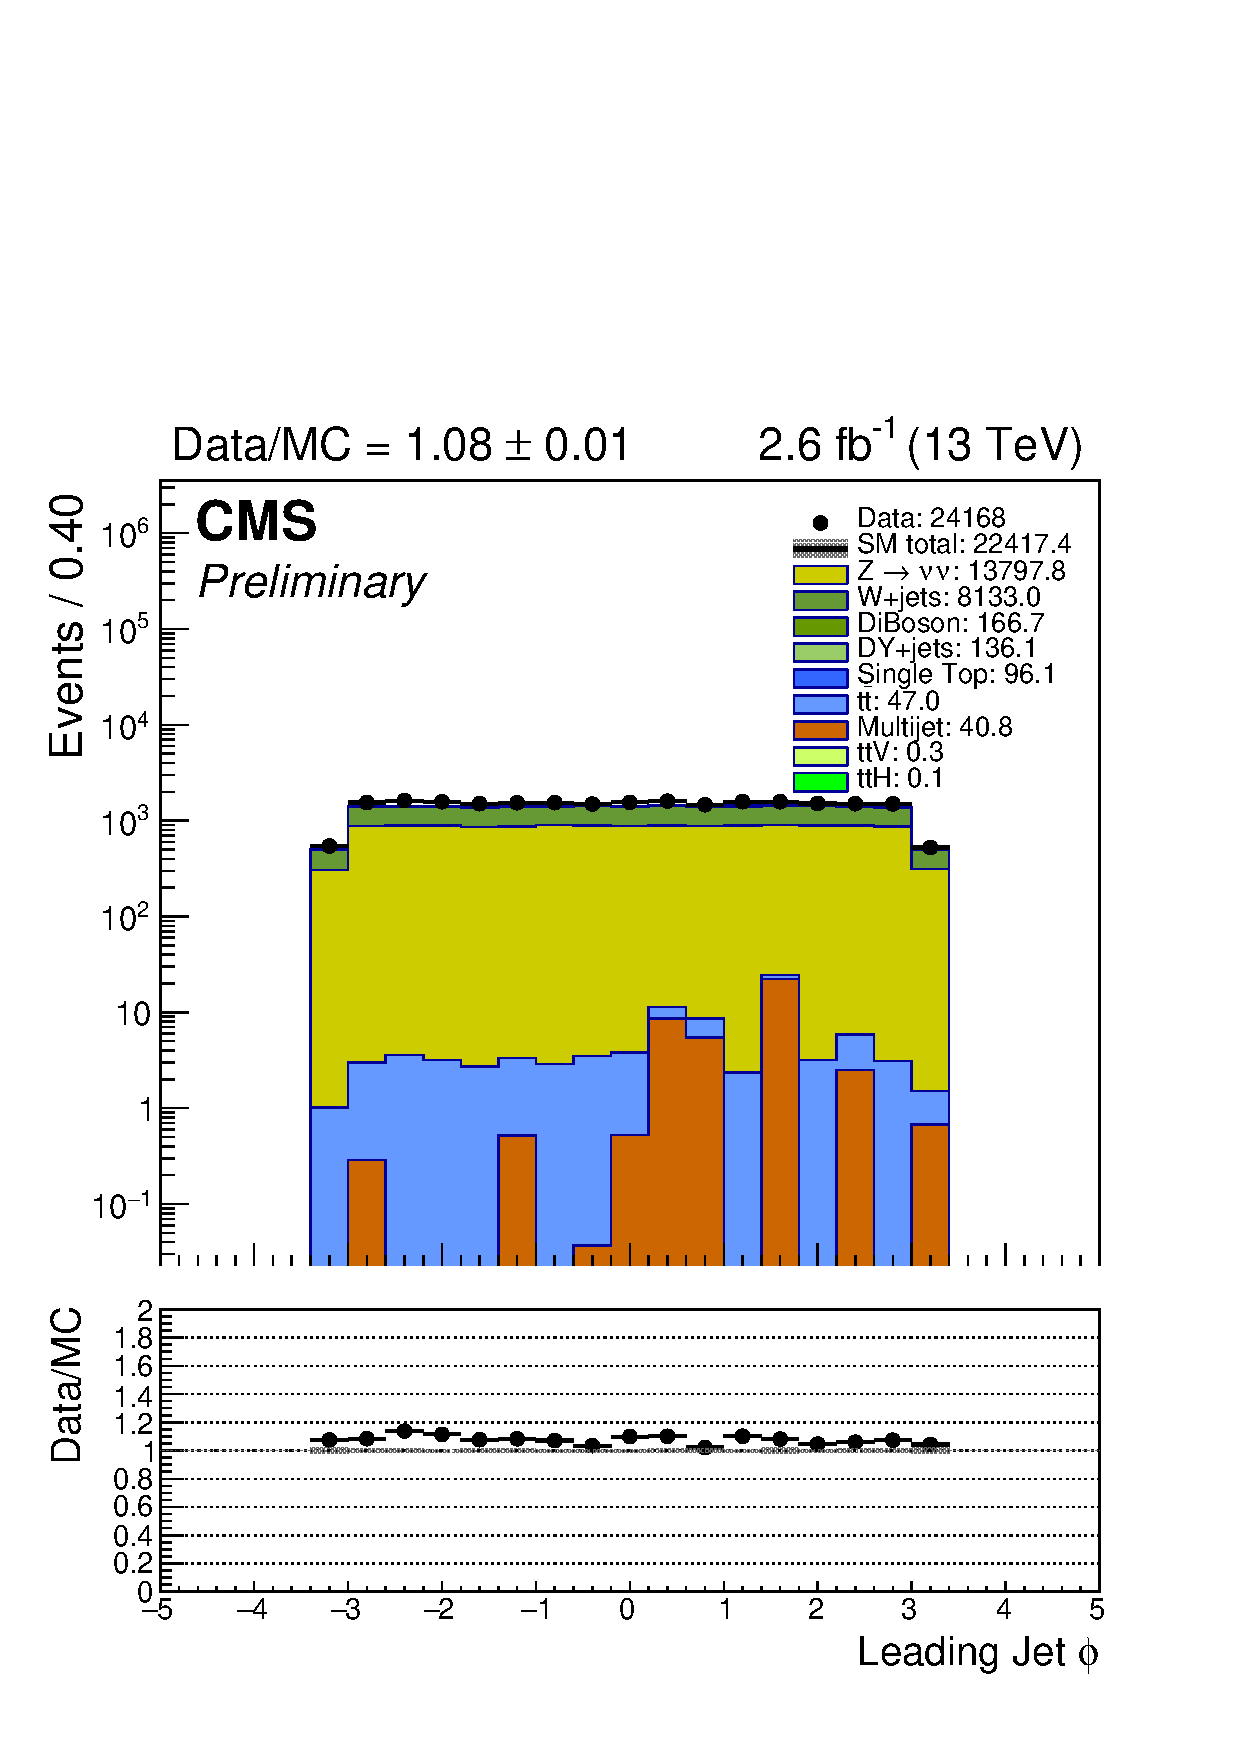
\includegraphics[width=0.32\textwidth]{figures/selection/jet_phi[0]_mono_all_after.pdf}}
        \caption{Distributions in the signal region of the jet charged hadron
        energy fraction (CHF) (Left), jet $\phi$ direction (Centre), and jet $\phi$
        direction after applying a requirement of {CHF~$>0.1$}. The large excess in data
        at charged hadron fractions close to zero and ${\phi = 0, \pi}$ is consistent with beam
        halo effects, and is effectively suppressed by the aforementioned selection.}
        \label{fig:leadJetCleaning}
    \end{center}
\end{figure}


\subsubsection{Summary of signal region selection} 
\label{sec:summary-selection}

The requirements that define the hadronic signal region are summarised
in Table~\ref{tab:sr-selections}.

\begin{table}[h!]
  \topcaption{Summary of the signal region selection criteria, applied
    in addition to the pre-selection summarised in
    Table~\ref{tab:pre-selections}.}
  \label{tab:sr-selections}
  \centering
  \footnotesize
  \begin{tabular}{ ll }
    \hline
    \hline
    Selection             & Requirement                                                    \\    
    \hline
    Veto                  & Veto on leptons, photons and SITs                              \\
    \alphat               & $>$0.52--0.65 (\HT-dependent) for region $200 < \HT < 900\gev$ \\
    \bdphi                & $>0.5$                                                         \\
    ``Beam Halo Filter''  &  $CHF(\textrm{leading jet})>0.1$                                \\
      &  $CHF(\textrm{leading jet})<0.95$                                \\
    \hline
    \hline
  \end{tabular}
\end{table}


\subsection{The control regions}
\label{sec:control-region-selection}


\subsubsection{The \texorpdfstring{\mj}{muon plus jets} control sample}
\label{sec:mucontrolSelection}

The selection criteria for the \mj sample are chosen to identify W
bosons decaying to a muon and a neutrino in the phase-space of the
signal. In order to select events containing W bosons, exactly one
tight isolated muon (defined in Sec.~\ref{sec:muon-id}) within an acceptance of \PT $>$ 30 \gev and
$|\eta| <$ 2.1 is required. The muons is removed from the event while computing the \met-based quantities, like \mht, \alphat. 
The transverse mass of the W candidate must satisfy $30 < \mt(\mu,\pfmet) < 125\gev$. 
This cut is also effective in reducing potential signal contamination 
for final states with leptons. 
Events are vetoed if $\Delta R(\mu,\textrm{jet}) < 0.5$ for at least one jet. 

Events are vetoed if well-reconstructed, isolated electrons and
photons, defined in Sec.~\ref{sec:objects}, are found to be within the
acceptances defined in Sec.~\ref{sec:vetoes}. Hence the vetoes mirror
exactly those used in the signal region, except for the selected
muon. Similarly, events containing single isolated tracks are also
vetoed according to the object and acceptance definitions found in
Secs.~\ref{sec:objects} and~\ref{sec:vetoes}. All single isolated
tracks in the event are considered, except for that associated with
the identified, isolated muon.

\subsubsection{The \texorpdfstring{\mmj}{di-muon plus jets} control sample}
\label{sec:mumucontrolSelection}

The selection criteria are identical to those for the \mj sample, with
the following exceptions that are tuned to identify Z bosons decaying
to two muons in the kinematic phase space of the signal region. 
In order to select an event sample containing Z bosons, exactly two
tight isolated muons (defined in Sec.~\ref{sec:muon-id}) within an acceptance of $\Pt > 30\gev$ and
$|\eta| < 2.1$ are required. The two muons are required to have opposite electric charge 
and the invariant mass of the two muons must satisfy $m_{Z} - 25 < M_{\mu_1\mu_2} < m_{Z} +25$. 
Events are vetoed if $\Delta R(\mu,\textrm{jet}) < 0.5$ is satisfied, running over all muons
and all jets. 

Events are vetoed if well-reconstructed, isolated electrons and
photons, defined in Sec.~\ref{sec:objects}, are found to be within the
acceptances defined in Sec.~\ref{sec:vetoes}. Hence the vetoes mirror
exactly those used in the signal region, except for the selected
muons. Similarly, events containing single isolated tracks are also
vetoed according to the object and acceptance definitions found in
Secs.~\ref{sec:objects} and~\ref{sec:vetoes}. All single isolated
tracks in the event are considered, except for that associated with
the identified, isolated muons.

\subsubsection{The \texorpdfstring{\gj}{photon plus jets} control sample}
\label{sec:photoncontrolSelection}

The \gj sample is defined by requiring exactly one photon (defined in Sec.~\ref{sec:photon-id}) satisfying
tight isolation criteria and within an acceptance of $\pt > 200\gev$
(limited by trigger requirements) and $|\eta| < 1.45$. Furthermore,
events are vetoed if $\Delta R(\gamma,\textrm{jet}) < 1.0$ is
satisfied for at least one jet. One important difference with
respect to the leptonic control samples is the application of the
\HT-dependent \alphat requirements imposed as part of the signal
region definition. This is done primarily to ensure that the photon
control sample and signal region are subject to identical kinematic
requirements and the photon carries sufficient transverse energy so
that the mass of the Z boson becomes a negligible effect when using
the \gj sample to predict the kinematic distributions of the \znunu
background. 

Events are vetoed if well-reconstructed, isolated muons and electrons,
defined in Sec.~\ref{sec:objects}, are found to be within the
acceptances defined in Sec.~\ref{sec:vetoes}. Hence the vetoes mirror
exactly those used in the signal region, except for the selected
photon. Similarly, events containing single isolated tracks are also
vetoed according to the object and acceptance definitions found in
Secs.~\ref{sec:objects} and~\ref{sec:vetoes}. 

\subsection{Event categorisation}
\label{sec:event-categorisation}

The events in the signal region and control regions are categorised according to 
\njet, \nb and \scalht. 
The categorisation in the control region ``mirrors'' the one in the search region: 
as a result no extrapolation is performed in these variables when predicting the backgrounds. \\
The bins used in the signal region are the result of an aggregation of the finer control region bins, 
with each of multiple control region bins predicting separately a category of events in the same aggregate bin in the signal region. 
This scheme, which is fully implemented in the likelihood as described in Sec. \ref{sec:likelihood}, allows 
to avoid any extrapolation while reducing the number of search categories. \\
The \textit{nominal} binning for these variables is summarised in Tab.~\ref{tab:nominal-binning}. 

\begin{table}[h!]
  \topcaption{Summary of the nominal \njet, \nb, \scalht binning.}
  \label{tab:nominal-binning}
  \centering
  \begin{tabular}{ cl }
    \hline
    \hline
    \multicolumn{2}{c}{Signal region} \\
    \hline
    Variable & Binning \\
    \hline
    \multirow{3}{*}{\njet}
     & Monojet:    $\njet=1$ \\
     & Asymmetric: $\njet \geq 2$ \\
     & Symmetric:  $\njet =2,3,4,5 \geq 6$ \\
    \hline
    \nb & $\nb=0,1,2,3,\geq 4$ \\
    \hline
    \scalht (GeV) & (200,400), (400,600), (600,900), (900,1200), $>$1200 \\
    \hline
    \hline
    \multicolumn{2}{c}{Control regions} \\
    \hline
    Variable & Binning \\
    \hline
    \multirow{3}{*}{\njet}
     & Monojet:    $\njet=1$ \\
     & Asymmetric: $\njet=2,3,4, \geq 5$ \\
     & Symmetric:  $\njet =2,3,4,5 \geq 6$ \\
    \hline
    \nb & $\nb=0,1,2,3,\geq 4$ \\
    \hline
    \scalht (GeV) & \parbox[t]{12cm}{(200,250), (250,300), (300,350), (350,400),
      (400,500), (500,600), \\ (600,750), (750,900), (900,1050), (1050,1200), $>$1200 } \\
    \hline
    \hline
  \end{tabular}
\end{table}


Starting from the definition of nominal binning, it has to be remarked that not all the (\njet,\nb,\scalht) combinations 
are kinematically accessible. For example, no $\njet=2,\nb=3$ bin exists (due to the jet multiplicity constraint) 
or $\njet^{sym} \geq 6,\scalht<400\,\mathrm{GeV}$ (due to jet acceptance requirements). 

Moreover, a requirement is made in order to ensure a reasonable number of events is available in data 
in each (\njet,\nb,\scalht) bin for the background prediction. 
A minimum of 10 events in every bin is required for at least one of the 3 control regions (\mj,\mmj,\gj). 

In order to improve the sensitivity to the signal, the search region is also binned in the \MHT dimension. 
Simulation mismodelling in this variable is reduced by binning the control regions finely in \scalht, i.e. by predicting 
events at the same ``scale''. A careful validation of the \MHT shape is carried out to assess 
the uncertainty in this extrapolation and it's described in Sec.~\ref{sec:syst-on-shape}. 

The \MHT templates which are used in the likelihood fit are built
using a minimum bin width of 100 GeV for $\MHT<400$ GeV and 200 GeV
above. The lowest nominal bin is $130<\MHT<200\,\mathrm{GeV}$. The
\MHT templates are naturally bounded from above by \scalht, apart from
the last open \scalht bin. However, the lower bound of the last open
bin is limited to $\MHT>1000\,\mathrm{GeV}$, to ensure sufficient data
counts in the control regions to validate the modelling at high \mht. 
Starting from this nominal binning, a requirement is made to ensure
that each bin in the template is well populated in the simulation.  At
least 100 unweighted MC events are required in each \njet,\scalht,\MHT
bin (inclusive in \nb). Adjacent \mht bins are merged until this
requirement is satisfied. 

The binning of the \MHT templates derived using these metrics is summarised in Tab.~\ref{tab:mht-binning}.


\newpage
\begin{table}[h!]
  \topcaption{Summary of the \MHT binning in each signal region
    category, determined according to the metrics described in this Section. The \MHT binning is identical in each \nb bin by construction.}
  \label{tab:mht-binning}
  \centering
  \begin{tabular}{ ccll }
    \hline
    \hline
    \njet & \nb & \scalht & \MHT \\
    \hline
    \multirow{4}{*}{$n_{\mathrm{jet}} = 1$} & \multirow{4}{*}{all} & [200,400] & [200,300], [300,inf] \\      
    & & [400,600] & [400,inf] \\ 
    & & [600,900] & [600,800], [800,inf] \\ 
    & & [900,inf] & [900,inf] \\     
    \hline
    \multirow{4}{*}{$n^{asym}_{\mathrm{jet}} \geq 2$} & \multirow{4}{*}{all} & [200,400] & [130,200], [200,300], [300,inf] \\
    & & [400,600] & [130,200], [200,300], [300,500], [500,inf] \\
    & & [600,900] & [130,400], [400,600], [600,800], [800,inf] \\
    & & [900,inf] & [130,800], [800,1000], [1000,inf] \\
    \hline
    \multirow{5}{*}{$n^{\mathrm{sym}}_{\mathrm{jet}} = 2$} & \multirow{5}{*}{all} & [200,400] & [130,200], [200,300], [300,inf] \\
    & & [400,600] & [130,200], [200,300], [300,500], [500,inf] \\
    & & [600,900] & [130,300], [300,400], [400,600], [600,800], [800,inf] \\
    & & [900,1200] & [130,300], [300,400], [400,600], [600,800], [800,1000], [1000,inf] \\
    & & [1200,inf] & [130,400], [400,600], [600,800], [800,1000], [1000,inf] \\
    \hline
    \multirow{5}{*}{$n^{\mathrm{sym}}_{\mathrm{jet}} = 3$} & \multirow{5}{*}{all} & [200,400] & [130,200], [200,300], [300,inf] \\    
    & & [400,600] & [130,200], [200,300], [300,500], [500,inf] \\
    & & [600,900] & [130,300], [300,500], [500,700], [700,inf] \\
    & & [900,1200] & [130,300], [300,400], [400,600], [600,800], [800,1000], [1000,inf] \\
    & & [1200,inf] & [130,400], [400,600], [600,800], [800,1000], [1000,inf] \\
    \hline
    \multirow{5}{*}{$n^{\mathrm{sym}}_{\mathrm{jet}} = 4$} & \multirow{5}{*}{all} & [200,400] & [130,200], [200,300], [300,inf] \\
    & & [400,600] & [130,200], [200,300], [300,500], [500,inf] \\
    & & [600,900] & [130,200], [200,300], [300,500], [500,700], [700,inf] \\
    & & [900,1200] & [130,300], [300,400], [400,600], [600,800], [800,1000], [1000,inf] \\
    & & [1200,inf] & [130,300], [300,400], [400,600], [600,800], [800,1000], [1000,inf] \\
    \hline
    \multirow{5}{*}{$n^{\mathrm{sym}}_{\mathrm{jet}} = 5$} & \multirow{5}{*}{all} & [200,400] & [130,200], [200,inf] \\
    & & [400,600] & [130,200], [200,300], [300,400], [400,inf] \\
    & & [600,900] & [130,300], [300,500], [500,700], [700,inf] \\
    & & [900,1200] & [130,300], [300,500], [500,700], [700,900], [900,inf] \\
    & & [1200,inf] & [130,300], [300,400], [400,600], [600,800], [800,1000], [1000,inf] \\
    \hline
    \multirow{4}{*}{$n^{\mathrm{sym}}_{\mathrm{jet}} \geq 6$} & \multirow{4}{*}{all} & [400,600] & [130,200], [200,300], [300,inf] \\
    & & [600,900] & [130,300], [300,400], [400,600], [600,inf] \\
    & & [900,1200] & [130,200], [200,300], [300,400], [400,600], [600,800], [800,inf] \\
    & & [1200,inf] & [130,300], [300,400], [400,600], [600,1000], [1000,inf] \\
    \hline
    \hline
  \end{tabular}
\end{table}
